\input{./_path-to-root.ltx}
\documentclass[\PathToRoot/\ProjectName]{subfiles}
\whenstandalone{\externaldocument{\PathToRoot/\ProjectName}}

\begin{document}

\begin{figure}[H]
  \centering
  \caption{Model validation for non-targeted spending patterns}
  \whenintegrated{\label{fig:untargetedMoments}} 
  \noindent\begin{minipage}{\textwidth}
    \centering
    \begin{subfigure}[b]{.48\linewidth}
      \centering
      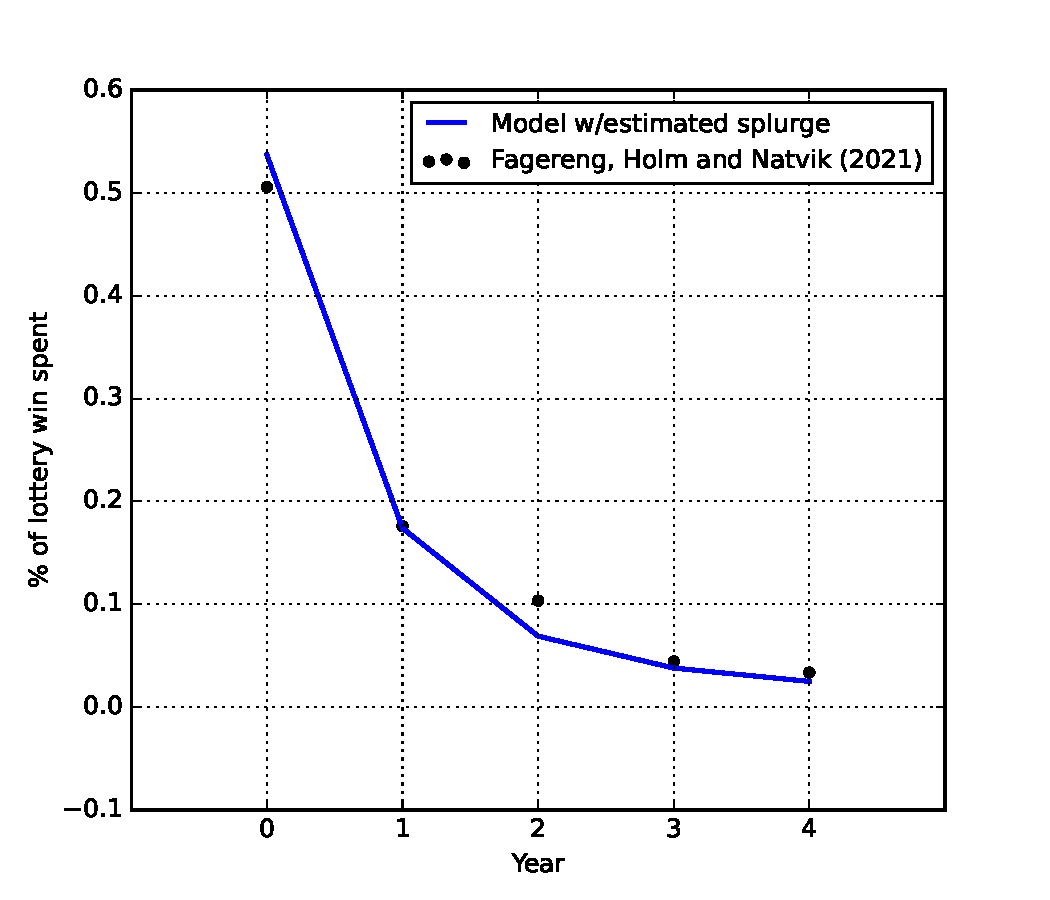
\includegraphics[width=\linewidth]{\PathToRoot/images/IMPCs_wSplEstimated}
      \caption{Dynamic spending after lottery win}
      \whenintegrated{\label{fig:USaggmpclotterywin}} 
    \end{subfigure}
    %
    \begin{subfigure}[b]{.48\linewidth}
      \centering
      % Original path: \PathToRoot/Code/HA-Models/FromPandemicCode/Figures/UnempSpell_Dynamics
      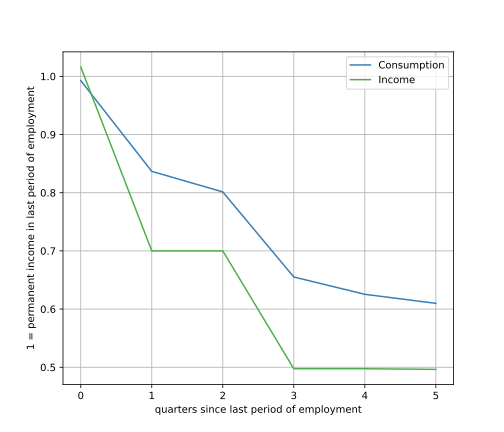
\includegraphics[width=\linewidth]{\PathToRoot/images/UnempSpell_Dynamics}
      \caption{Spending upon UI benefit expiry}
      \whenintegrated{\label{fig:expiryUI}} 
    \end{subfigure}
  \end{minipage}
\end{figure}
\noindent\parbox{\textwidth}{\footnotesize
  \textbf{Note}: This figure demonstrates model performance on non-targeted validation moments (Section~\ref{sec:nonTargetedMoments}).
  Subfigure~(a) shows the model's dynamic consumption response compared to \cite{fagereng-mpc-2021} estimates
  using the discount factor distributions estimated separately for each education group.
  Subfigure~(b) validates the model against \cite{ganongConsumer2019}, who find that nondurable spending
  drops by 12\% the month when UI benefits expire; our quarterly model predicts an 18\% drop
  the quarter after benefit expiry,   demonstrating broad consistency with this empirical pattern.
}

\vspace{1em}  % Add space after figure

% Smart bibliography: Only include bibliography if standalone AND has citations
\smartbib

\end{document}
